\documentclass{article}
\usepackage[utf8]{inputenc}
\usepackage[russian]{babel}
%\usepackage{systeme}
\usepackage{amsmath}
\usepackage{amssymb}
\usepackage{amsfonts}
\usepackage{mathtext}

\usepackage[final]{graphicx}
\graphicspath{{noiseimages/}}

\renewcommand{\baselinestretch}{1.5}

\title{Шестое задание БМСО}
\author{Ярослав Аверьянов}
\date{Декабрь 2015}

\begin{document}

\maketitle

\section{Первая задача}
Рассматривается алгоритм сэмплирования Гиббса из распределения $p(x_1,...,x_n)$.\\
a) Покажем, что $p^{*}(x_i)q(x_i|x_j) = p^{*}(x_j)q(x_i|x_j);i,j = 1,...,n$\\
Здесь $q(x^{k+1},x^{k})$ - распределение значений на $k + 1$ шаге при заданном значении на $k$ шаге.\\
Далее будет использоваться обозначение $\theta = x$.(векторно)\\
Тогда для сэмлирования Гиббса функцию переходных вероятностей нужно взять следующим образом:\\
$J_{j,t}^{Gibbs}(\theta^{t}|\theta^{t-1}) = p(\theta_j^{t}|\theta_{-j}^{t-1})$, если $\theta_{-j}^{t} = \theta_{-j}^{t-1}$.\\
Далее рассмотрим следующий коэффицент:\\
$r = \frac{\frac{p(\theta^{t})}{J_{j,t}^{Gibbs}(\theta^{t}|\theta^{t-1})}}{\frac{p(\theta^{t-1})}{J_{j,t}^{Gibbs}(\theta^{t-1}|\theta^{t})}} = \frac{\frac{p(\theta^{t})}{p(\theta_{j}^{t}|\theta_{-j}^{t-1})}}{\frac{p(\theta^{t-1})}{p(\theta_{j}^{t-1}|\theta_{-j}^{t-1})}} = \frac{p(\theta_{-j}^{t-1})}{p(\theta_{-j}^{t-1})} = 1.$\\
б) Построим алгоритм Метрополиса-Хастингса эквивалентный такому сэмплированию Гиббса:\\
1.Берем $\theta^{0}:p(\theta^{0}) > 0$.\\
2.Для $t = 1,...,T$ сэмплируем $\theta^{*}$ из распределения $J_{t}^{Gibbs}(\theta^{*}|\theta^{t-1})$, которое было определено в пунке a). Присваиваем $\theta^{t} = \theta^{*}$.


\section{Вторая задача}
Пусть есть $p(x_1,x_2) = Cexp(-x_1^2x_2^2);$\\
Будем исходить из сэмплирования Гиббса:\\
1.Берем $x^{(0)}:p(x^{(0)}) > 0;$\\
2.Повторяем $t = 1,2,...,T:$\\
a)$x_1^{(t)} \sim p(x_1|x_2^{(t-1)});$\\
б)$x_2^{(t)} \sim p(x_2|x_1^{(t)});$\\
В результате $(x_1^{(1)}, x_2^{(1)}),...,(x_1^{(T)}, x_2^{(T)})$ из $p(x_1,x_2);$\\
Здесь используется:\\
$p(x_1|x_2) \sim exp(-x_1^2x_2^2):\int_{-\infty}^{+\infty} exp(-x_1^2x_2^2)dx_1 = 1 \to p(x_1|x_2) \sim N(0,\sigma^2), \sigma = \frac{1}{\sqrt{2}x_2};$\\
$p(x_2|x_1) \sim exp(-x_1^2x_2^2):\int_{-\infty}^{+\infty} exp(-x_1^2x_2^2)dx_2 = 1 \to p(x_2|x_1) \sim N(0, \sigma^2), \sigma = \frac{1}{\sqrt{2}x_1};$\\
Численная реализация проведена в python notebook.\\
$N = 300, x^{0} = 0.5, y^{0} = 0.5$
\begin{figure}[h]
\center{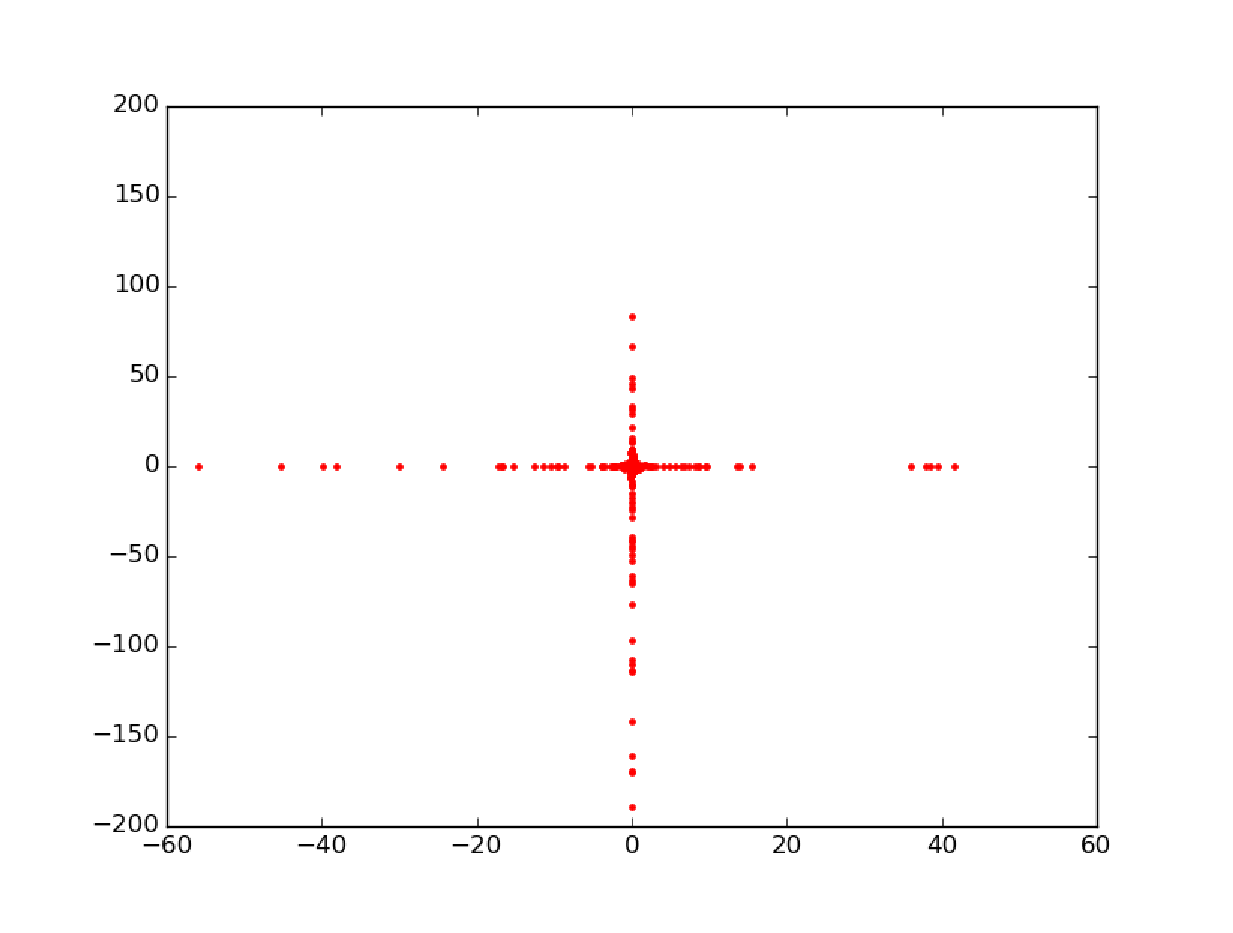
\includegraphics[width=0.5\linewidth]{figure_2}}
\caption{Gibbs sampling for $p(x_1, x_2) \sim exp(-x_1^2x_2^2)$}
\label{ris:image}
\end{figure}



\section{Третья задача}
$X_1 \sim Gamma(\alpha_1) \quad X_2 \sim Gamma(\alpha_2)$\\
$X_1$ и $X_2$ - независимые СВ.\\

Необходимо показать, что $X_1 + X_2$ и $\frac{X_1}{X_1 + X_2}$ - независимые СВ\\
Пусть $Y_1 = \frac{X_1}{X_1 + X_2} = g_1(X_1,X_2), \qquad Y_2 = X_1 + X_2 = g_2(X_1,X_2)$\\
$X_1 = Y_1Y_2$\\
$X_2 = Y_2(1 - Y_1)$\\
Якобиан замены:$\quad J = det((X_1,X_2) \to (Y_1,Y_2)) = Y_2;$\\

$f_{X_1,X_2}(x_1,x_2) = \frac{1}{\Gamma(\alpha_1)\Gamma(\alpha_2)}x_1^{\alpha_1 - 1}x_2^{\alpha_2 - 1}exp(-(x_1+x_2)),$ при $x_1,x_2 > 0$ - совместное распределение $(X_1,X_2)$\\
Найдем совместное распределение $Y_1$ и $Y_2$:\\
$f_{Y_1,Y_2}(y_1,y_2) = f_{X_1,X_2}(g_1^{-1}(y_1,y_2),g_2^{-1}(y_1,y_2))|J| = \frac{1}{\Gamma(\alpha_1)\Gamma(\alpha_2)}(y_1y_2)^{\alpha_1 - 1}(y_2(1-y_1))^{\alpha_2-1}exp(-y_2)|y_2|,$ если $0 < y_1 < 1, y_2 > 0$\\
\\
$f_{Y_1}(y_1) = \frac{1}{\Gamma(\alpha_1)\Gamma(\alpha_2)}\int_0^\infty (y_1y_2)^{\alpha_1 - 1}(y_2(1-y_1))^{\alpha_2 - 1}e^{-y_2}|y_2|dy_2 = \frac{1}{\Gamma(\alpha_1)\Gamma(\alpha_2)}\int_0^\infty y_2^{\alpha_1 + \alpha_2 -1}e^{-y_2}y_1^{\alpha_1 - 1}(1-y_1)^{\alpha_2 - 1}dy_2 = \frac{\Gamma(\alpha_1 + \alpha_2)}{\Gamma(\alpha_1)\Gamma(\alpha_2)}y_1^{\alpha_1 - 1}(1-y_1)^{\alpha_2 - 1}, 0 < y_1 < 1$\\
Также $X_1 + X_2 \sim Gamma(\alpha_1 + \alpha_2) \sim \frac{1}{\Gamma(\alpha_1 + \alpha_2)}x^{\alpha_1 + \alpha_2 - 1}e^{-x}, \quad x \geq 0$\\
Посмотрим выполнение равенства $p(y_1,y_2) = p(y_1)p(y_2):$\\
$f_{Y_1}(y_1)f_{Y_2}(y_2) = \frac{\Gamma(\alpha_1 + \alpha_2)}{\Gamma(\alpha_1)\Gamma(\alpha_2)}y_1^{\alpha_1 - 1}(1 - y_1)^{\alpha_2 - 1}\frac{1}{\Gamma(\alpha_1 + \alpha_2)}y_2^{\alpha_1 + \alpha_2 - 1}e^{-y_2} = \frac{1}{\Gamma(\alpha_1)\Gamma(\alpha_2)}y_1^{\alpha_1 - 1}y_2{\alpha_1 - 1}y_2^{\alpha_2}(1 - y_1)^{\alpha_2 - 1}e^{-y_2}$.\\
Равенство выполняется => верно.

\section{Четвертая задача}
В урне $c$ различных цветов и $\alpha(i) > 0$ - шаров $i^{го}$ цвета.\\
$k^{ый}$ шаг - достается цвет $x_k$, в урну кидается 2 шара цвета $x_k$ => выборка $(X_1,...,X_n)$.\\
Показать, что эти СВ - перестановочны.
\\
Рассмотрим следующие вероятности:\\
$\mathbf{P}[X_1 = j] = \frac{\alpha(j)}{\sum\limits_{i=1}^n \alpha(i)}$ \\
\\
$\mathbf{P}[X_2 = j|X_1] = \frac{\alpha(j) + [X_1 = j]}{\alpha(\mathbf{X}) + 1}$\\
--------------------------------------------------------------\\
$\mathbf{P}[X_1,X_2,...,X_n] = \mathbf{P}[X_1]\mathbf{P}[X_2|X_1]\mathbf{P}[X_3|X_2]...\mathbf{P}[X_n|X_{n-1}] = \frac{\alpha(x_1)}{\alpha(\mathbf{X})}\frac{\alpha(x_2) + [X_1 = x_2]}{\alpha(\mathbf{X})+1}....\frac{\alpha(x_n) + \sum\limits_{i=1}^{n-1}[X_i = x_n]}{\alpha(\mathbf{X}) + (n-1)}$\\
Т.к. полная вероятность предствлена в виде, который указан сверху, то при любой перестановке $(i_1,...,i_n)$ верно $\mathbf{P}[X_1,X_2,...,X_n] = \mathbf{P}[X_{i_1},X_{i_2},...,X_{i_n}]$. 


\end{document}
